\documentclass[11pt,twoside,letterpaper,onecolumn,english]{article}
\input{my_style}

%\documentclass[modern]{desc-tex/styles/lsstdescnote}

% LATEX PACKAGES
%\usepackage{desc-tex/styles/lsstdesc_macros}

\usepackage{xcolor}
\usepackage{authblk}

\begin{document}
\markboth{Photometric Redshift Ensemble (NZ) Data Challenge}{Photometric Redshift Ensemble (NZ) Data Challenge}

\title{Photometric Redshift Data Challenge}
\author[1,2]{Eric Charles}
\author[3]{Qianjun Hang}
\author[4]{Josue De Santiago}
\author[5]{Leonel Media-Varela}
\author[6]{Justin Myles}
\author[7]{Samuel J.  Schmidt}
\author[1,2]{Tianqing Zhang}
\affil[1]{\small SLAC National Accelerator Laboratory, 2575 Sand Hill Road, Menlo Park, CA 94025, USA}
\affil[2]{Kavli Institute for Particle Astrophysics and Cosmology (KIPAC), Stanford University, Stanford, CA 94305, USA}
\affil[3]{Department of Physics \& Astronomy, University College London, Gower Street, London WC1E 6BT, UK}
\affil[4]{Secihti---Departamento de F\'isica, Centro de Investigaci\'on y de Estudios Avanzados del I.P.N. Apdo. 14-740, Ciudad de M\'exico 07000, M\'exico}
\affil[5]{McWilliams Center for Cosmology and Astrophysics, Department of Physics, Carnegie Mellon University, Pittsburgh, PA, USA}
\affil[6]{Department of Astrophysical Sciences, Princeton University, Princeton, NJ 08544, USA}
\affil[7]{Department of Physics and Astronomy, University of California, One Shields Avenue, Davis, CA 95616, USA}
\date{\today}

\maketitle

\begin{abstract}
  Many Rubin science cases will require determining the 
  redshift distribution $n(z)$ for ensembles of objects, e.g., all the
  galaxies assigned to a particular tomographic bin in a cosmology analysis.
  We are organizing an NZ data challenge, following
  on from a PZ data challenge that focused on per-object estimates ($p(z)$). 
  The goal of this challenge is to assess the current status of NZ algorithms and analysis pipelines.
  This document describes the format of the NZ challenge, including the
  data that participants will use, the tasks that they will
  be asked to perform, and the metrics and criteria by which submissions will
  be assessed. It also provides detailed instructions for how to
  submit entries to the challenge.  
\end{abstract}


\section{Introduction}
\label{sec:intro}

Redshift inference is a key element of many DESC science
goals, and redshift uncertainty is one of the leading contributors to
the overall uncertainty on cosmological models from imaging survey
data.  Precursor surveys took a variety of approaches to this problem,
accounting for differences in underlying data as well as modeling
approaches.  In all cases, redshift uncertainty was significantly
larger than the requirements listed in the LSST DESC Science
Requirements Document.   

This state of the art motivates a data challenge to characterize and
improve existing methods, as well as to provide infrastructure for the
development of improved methods. Overall, this requires generating
uniform input catalogs and infrastructure for comparing output
redshift posteriors for ensembles to each other and to simulated truth catalogs.

Estimating ensemble-level $n(z)$ distributions differs from measuring
per-object $p(z)$ distributions in many ways.  Depending on the method,
estimating $n(z)$ distributions may or may not include $p(z)$ estimation along the way.


\section{Photometric redshift basics}
\label{sec:redshift_basics}

Photometric redshift estimation involves taking a catalog of galaxies
for which we have observations in several different filters and have
measured the brightness of the galaxies in those bands, and
using that information to estimate the redshift of the galaxies.
For LSST we expect to have measurements in 6 bands: 'u', 'g', 'r',
'i', 'z', and 'y', covering a wavelength range from approximately 
320 to 1600 nanometers. For the Roman space telescope, this will
extend from about 500 to 2300 nanometers.

Much of the information used to estimate photometric redshifts derives
from the 'Balmer break' present in the rest frame of many spectra at
400 nm. As the break crosses into different optical filters with
increasing redshift, the differences in magnitudes between filters
carry information about the redshift; see, e.g.,
Fig.~\ref{fig:pz_redshift_basics}. This can also be seen when
plotting redshifts as a function of derived colors, i.e., differences
in magnitudes between filters; see, e.g., Fig.~\ref{fig:color_color_redshift}.

\begin{figure*}[ht]
  \centerline{
    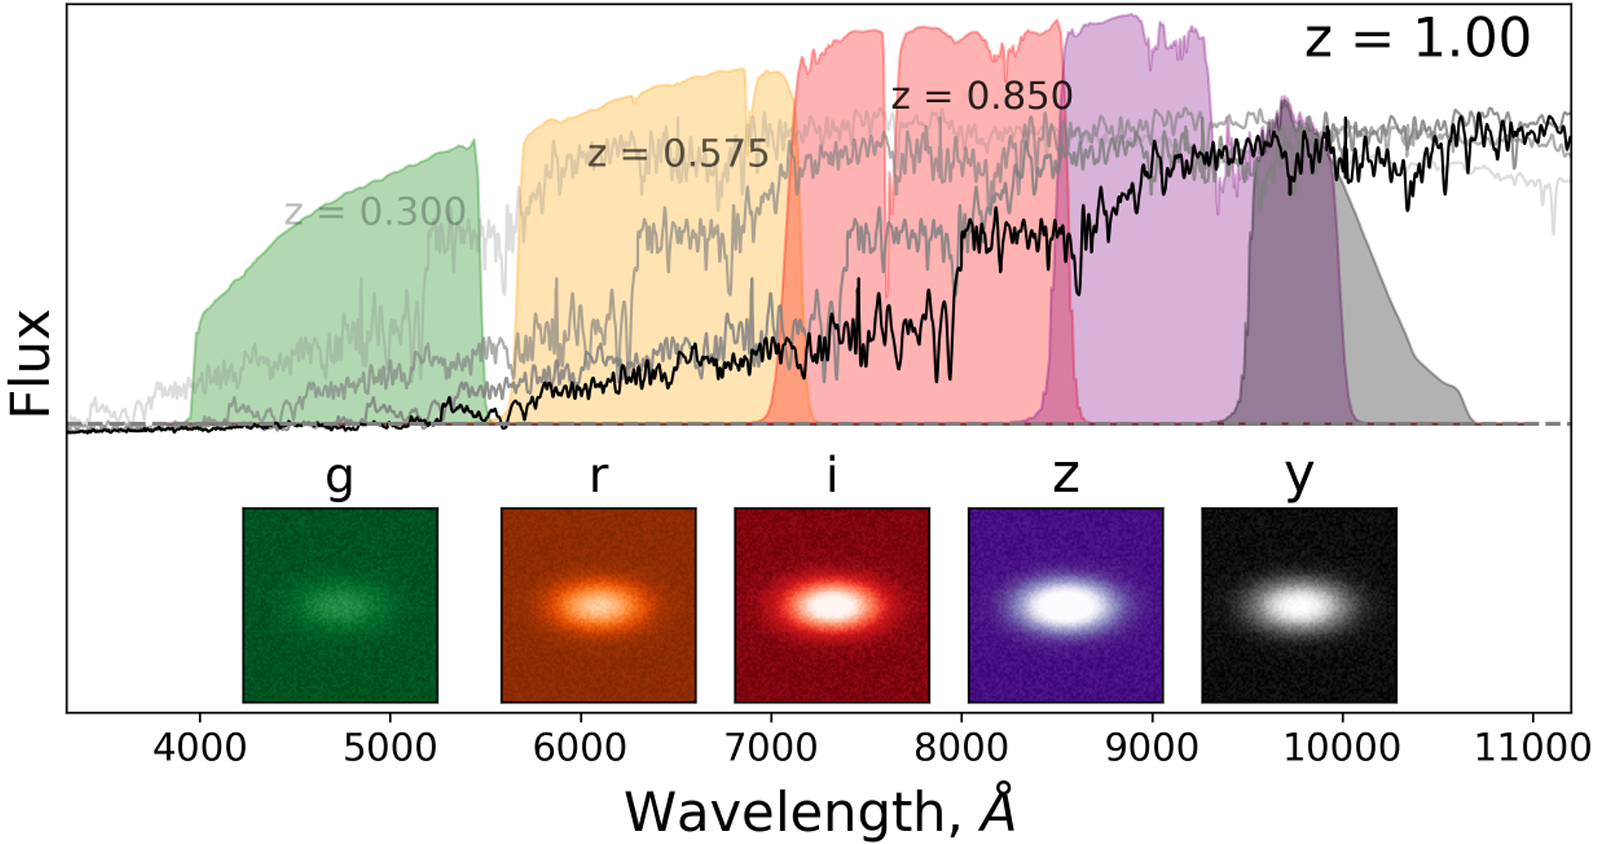
\includegraphics[width=0.80\textwidth]{figures/static_balmer.png}    
  }
  \caption{\label{fig:pz_redshift_basics}\small{A passive galaxy at
      different redshifts and how it will show up in various optical
      filters, giving us the ability to estimate its redshift and
      therefore distance. For many galaxies, the so-called
      'Balmer break' at 400 nm is a reliable feature that causes the
      flux to drop severely in bluer filters. Figure and caption
      by Jamie McCullough.}}
\end{figure*}

\begin{figure*}[ht]
  \centerline{
    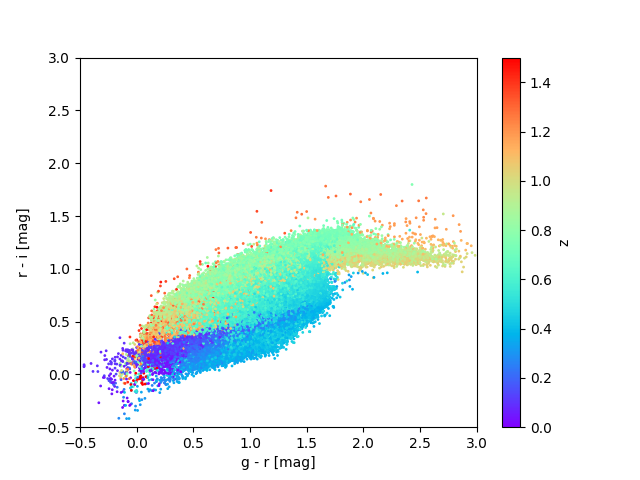
\includegraphics[width=0.45\textwidth]{figures/color_color_redshift_taskset_1_cardinal_10yr}    
    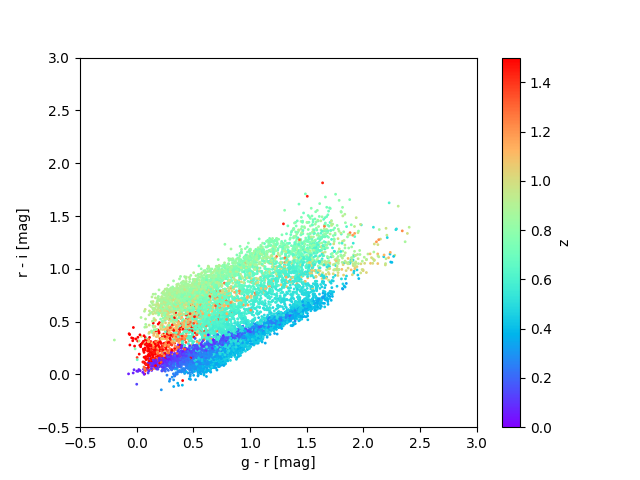
\includegraphics[width=0.45\textwidth]{figures/color_color_redshift_taskset_1_flagship_10yr}
  }
  \caption{\label{fig:color_color_redshift}\small{Redshifts plotted as
      a function of $r-i$ versus $g-r$ colors for a sample of objects
      in the cardinal (left) and flagship (right) simulations. These
      are plotted for the data for task set 1, i.e., for a sample of
      objects with $i < 23$.}}
\end{figure*}

This overly simple picture is complicated somewhat by the fact that
different galaxies have different intrinsic spectra and colors, as
seen in Fig.~\ref{fig:color_redshift}.

\begin{figure*}[ht]
  \centerline{
    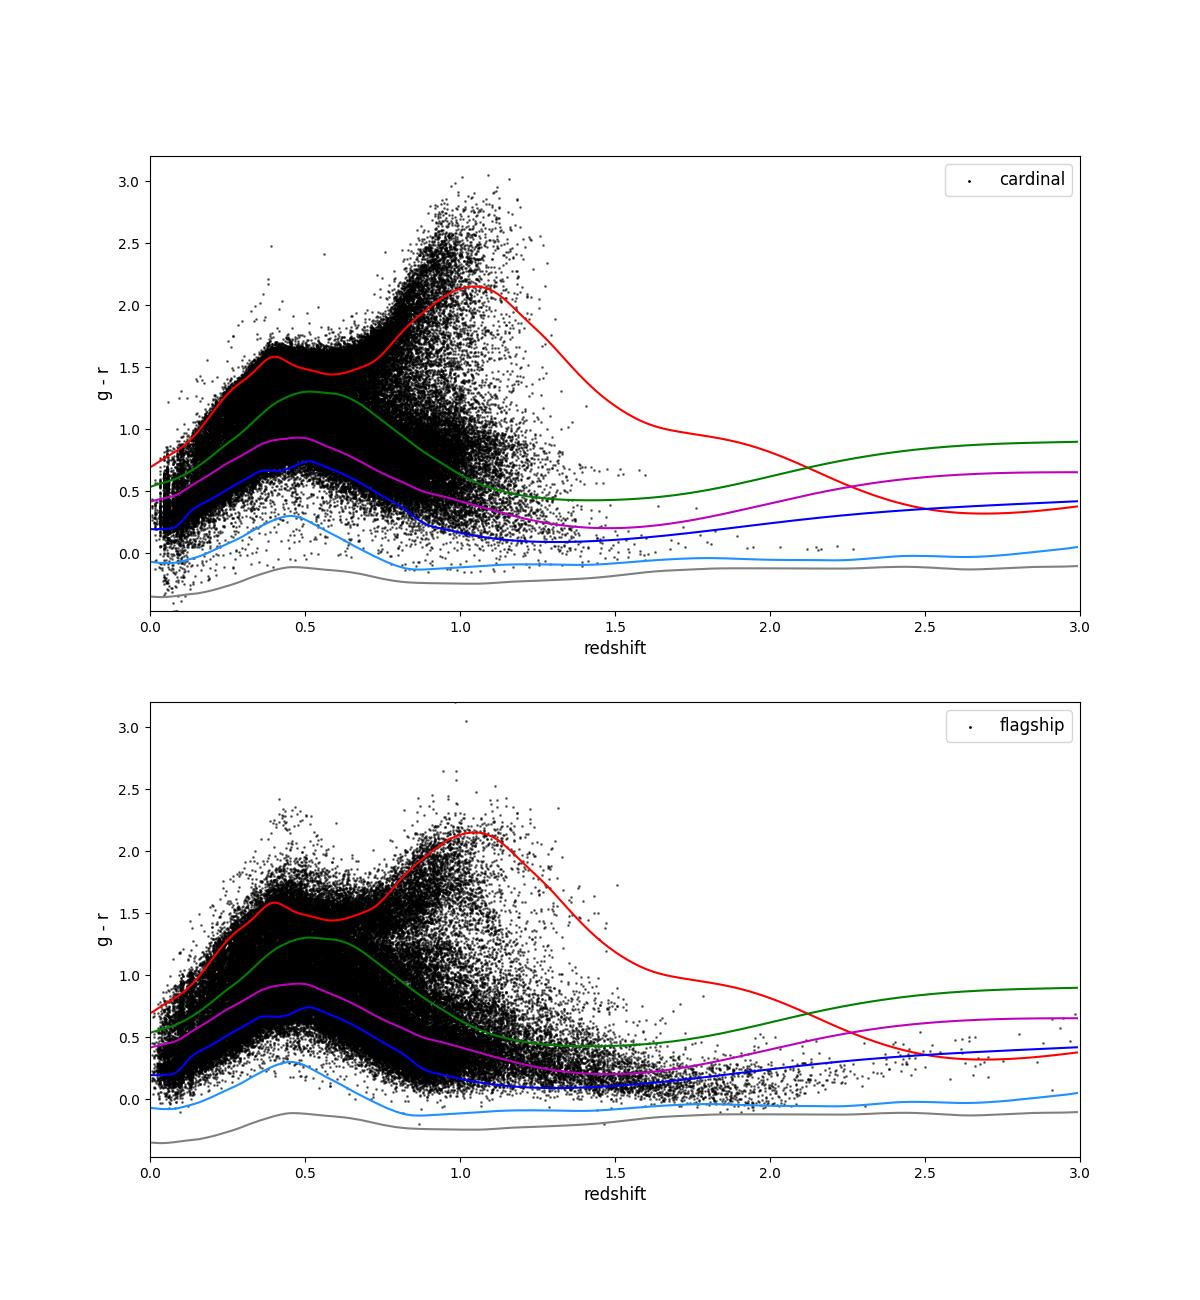
\includegraphics[width=0.80\textwidth]{figures/gr_vs_sz_sidebyside.jpg}    
  }
  \caption{\label{fig:color_redshift}\small{Color ($g-r$) plotted as a function of
      redshift for a sample of objects in the cardinal (top) and
      flagship (bottom) simulations. These are plotted for the data
      for task set 1, i.e., for a sample of objects with $i < 23$. The
      overlaid lines show the templates for several different types of galaxies.}}
\end{figure*}

This is further complicated by the fact that reference redshifts,
typically obtained by spectroscopy, slitless spectroscopy (i.e., grism
measurements), or multi-band photometric measurements, are not a
representative sample, as they are much easier to obtain for brighter
objects. Depending on the method used to obtain the reference
redshifts, they are also susceptible to errors such as confusing
different spectral lines or confusion of blended objects. Some of
the tasks in this data challenge encourage participants to try to
address these complications.


\section{Challenge Format}
\label{sec:challenge_format}

The NZ data challenge comprises a series of sets of tasks for participants.
Submissions will be evaluated to determine how ready various algorithms are
to be used for cutting-edge analysis based on how well they perform on
the various tasks. Readiness will be evaluated on a few different
fronts: 1) Does the algorithm meet performance requirements? 2) Is
it robust, flexible, and relatively easy to use on different datasets?
3) Is it scalable to the scales we will need?

This document and the associated web pages describe the data being
provided to participants, the tasks they will be asked to perform, the
expected format for submissions, and the metrics by which algorithm
readiness will be evaluated.


\subsection{Scope and Timeline}

The data challenge includes two major parts, with a set of
tasks emulating increasingly realistic scenarios in each part. The
percursor, ``PZ data challenge'', assessing per-object $p(z)$ estimation,
was launched in April 2026 and will conclude in September 2026.
The part desribed here, the ``NZ data challenge'', covering tomography and $n(z)$ estimation, will focus on assigning
objects to tomographic bins and estimating the distribution of redshifts in
each bin, and will launch in September 2026 and conclude in January 2027.

Preliminary results for the NZ part of the challenge 
with a technical note summarizing those results to follow shortly thereafter and
a comprehensive journal publication to follow later.


\subsection{Installing and setting up the \texttt{nz\_data\_challenge}
  package}

The \texttt{nz\_data\_challenge} package provides participants with tools
to access data, set up submissions, estimate performance metrics, and
format submissions.  It can be installed with a few small
variants on the standard \texttt{GitHub} package setup procedure.
Before starting, you should pick a name for your submission, e.g., ``example''.

\begin{verbatim}
# Create a conda environment
conda create --name nzdc python=3.13

# Clone the nz_data_challenge repository (or your fork of the repository)
git clone git@github.com:LSSTDESC/nz_data_challenge.git
# or git clone https://github.com/LSSTDESC/nz_data_challenge.git

# Go into the directory
cd nz_data_challenge

# Install the code in "editable" mode
pip install -e ".[dev]"

# Use the provided script to set up your submission.
# Here you should provide the name of your submission
python scripts/prepare_submission.py <submission_name>
\end{verbatim}

This final step will copy the input data files to
\texttt{nz\_data\_challenge/public}, and set up the three files you will
need to submit your entry.

The notebooks in the \texttt{nz\_data\_challenge/nb} area give examples
of how to access the data and create some of the diagnostic plots
that were used to validate the data.


\subsection{Submission mechanism}

Submissions will take the form of a pull request in the
\texttt{nz\_data\_challenge} repository.  Detailed instructions on how
to submit an entry are provided in
Sec.~\ref{sec:challenge_submissions} of this document.


\section{Challenge Input Data}
\label{sec:challenge_input_data}

The preparation of the challenge data is described in the appendices.
The data are available as a \texttt{tar} archive that is downloaded and
unpacked as part of the \texttt{nz\_data\_challenge} setup procedure.

Each task set in the data challenge has an associated set of files.
Typically these will be a collection of training files that contain
photometric data and reference redshifts, and a second set of files
that contain photometric data but do not include redshifts. Each
task set will involve estimating something about the redshifts or
redshift distributions in the test files.

Typically there will be several training and test files for a
particular task set, covering different scenarios and using different
input simulations.


\subsection{Input data format}

The input data for the challenge are presented in HDF5 files.
The naming convention for the files is
\texttt{\{challenge\}\_\{taskset\}\_\{simulation\}\_\{label\}\_\{scenario\}.hdf5}.
The meanings of the various \allowbreak fields are described in
Tab.~\ref{tab:file_fields}.   The various types of files are described in
Tab.~\ref{tab:file_types}. The columns in the files are described
in Tab.~\ref{tab:columns}.  We note that we use \texttt{np.nan} in
the magnitude columns to signify non-detections.

\begin{table}[ht]
\centering
\caption{\label{tab:file_fields}\small Fields in the input file names.}
\begin{tabular}{ll}
  \hline\hline  
  Field & Description \\ \hline
  challenge & Challenge associated with file (``nz\_challenge'') \\
  taskset & Task set associated with file (e.g., ``taskset\_1'') \\
  simulation & Simulation used to produce file (``cardinal'' or ``flagship'') \\
  label & File label (e.g., ``ddf\_03'', ``wfd'') \\
  scenario & Data scenario (e.g., ``1yr'', ``4yr''') \\
\hline\hline
\end{tabular}
\end{table}


\begin{table}[ht]
\centering
\caption{\label{tab:file_types}\small File Types.  The ``ddf\_00'' fields have reference redshifts
  from all spectroscopic samples.  The other ``ddf'' fields emulate the incomplete coverage coming only
  from the ``DESI'' samples.}
\begin{tabular}{ll}
  \hline\hline  
  Label & Description \\ \hline
  wfd & ``Wide, Fast, Deep'', emulating LSST and Roman survey data \\
  ddf\_00 & ``Deep-drilling field 0'', emulating COSMOS deep field. \\
  ddf\_0X & ``Deep-drilling field 1,2,3,4'', emulating other deep fields. \\  
\hline\hline
\end{tabular}
\end{table}


\begin{table}[ht]
\centering
\caption{\label{tab:columns}\small Contents of input files.}
\begin{tabular}{ll}
  \hline\hline
  Column & Description \\ \hline  
  redshift & True redshift (training files only) \\
  ra & Right ascension (training files only) \\
  dec & Declination (training files only) \\
  object\_id & Unique object ID\\
  mag\_\{band\}\_lsst & Magnitude in LSST \{band\} \\
  mag\_\{band\}\_lsst\_err & Magnitude uncertainty in LSST \{band\} \\
  mag\_\{band\}\_roman & Magnitude in Roman \{band\} \\
  mag\_\{band\}\_roman\_err & Magnitude uncertainty in Roman \{band\} \\
\hline\hline
\end{tabular}
\end{table}

We note that the \texttt{table-io} package~\cite{tables_io},
installed with \texttt{nz\_data\_challenge}, provides a command-line interface to
convert files from \texttt{hdf5} format to other formats such as
\texttt{parquet} tables or \texttt{pandas} data frames.

\begin{verbatim}
# convert a hdf5 file to pandas dataframe in a parquet file
tables-io convert
  --input public/nz_challenge_taskset_1_flagship_4yr_ddf_03.hdf5
  --output public/nz_challenge_taskset_1_flagship_4yr_ddf_03.pq
\end{verbatim}


\section{Challenge Submissions}
\label{sec:challenge_submissions}

\subsection{Challenge subtask types}

The challenge is organized as a series of sets of tasks using
increasingly realistic representations of the data. In general, each
set of tasks includes 3 subtasks.

\begin{enumerate}
\item{Provide tomographic bin assignments for all objects and estimate ensemble $n(z)$
      distributions for a set of different scenarios in a specified format.}
  \item{Provide trained models for the different scenarios and a
      Python function that can be used to generate the estimates from subtask
      1 on an arbitrary dataset.  We will not actually run these ourselves as part of the submisison validation,
      but will run them as part of the challenge.}
  \item{Provide a Python function that can be used to
      generate the models and estimates from subtasks 1 and 2 on
      arbitrary datasets.  Again, will not actually run these ourselves as part of the submisison validation,
      but will run them as part of the challenge.}
\end{enumerate}

The $n(z)$ estimates, bin assignments, and (for taskset 3) $n(z)$ samples
from subtask 1 should be provided in a compressed \texttt{tar} file.
A \texttt{timing.yaml} file is not required and is not checked by CI.
Any models used in subtask 2 should be provided in a separate \texttt{tar} file.
Templates and instructions for the Python functions needed for subtasks 2 and 3 are
described below. 

\subsection{Data format for submissions}

Each submisison will require creating a set of files described below and packaging them in a specific format.


\subsubsection{Data format for bin assignments}

The bin assignments should be provided as an HDF5 file containing a dictionary
with two arrays: object IDs (\texttt{object\_id}) and corresponding bin assignments (\texttt{tomo\_bin\_index}).  The tomographic
bins should run from 0 to $n_{\rm bins} -1$.  The value $-1$ is reserved as a guard
value for unassigned objects.  The files should be called, e.g., \texttt{nz\_challenge\_taskset\_1\_cardinal\_1yr\_bhat\_wfd.hdf5}.

Format tests do \textbf{not} read catalog IDs from the public WFD files.
\texttt{submit\_utils.check\_submission} currently compares \texttt{object\_id} to
sequential integers: taskset 1 starts at 0, tasksets 2 and 3 start at
4\,000\,000, then add 1\,000\,000 for each (simulation, scenario)
combination in the order cardinal/flagship $\times$ 1yr/4yr. Write those IDs
(not the simulation \texttt{object\_id} column) unless the validator is updated.

\begin{verbatim}
import numpy as np
import tables_io

n = 1_000_000
start = 0  # taskset_1_cardinal_1yr; see check_submission offsets
data_dict = dict(
    tomo_bin_index=bin_assignments,
    object_id=np.arange(start, start + n),
)
tables_io.write(data_dict, <output_filename.hdf5>)
\end{verbatim}



\subsubsection{\texorpdfstring{Data format for ensemble  $n(z)$ estimates}{Data format for ensemble n(z) estimates}}

The $n(z)$ estimates should be submitted in \texttt{qp} format,
which allows users to specify a complete $n(z)$ distribution for
each tomographic bin, as well as summary statistics for each ensemble.

The \texttt{qp} package~\cite{QP} supports several different representations of
$n(z)$, such as different functional forms as well as interpolated
grids, histograms, and others.

For users unfamiliar with \texttt{qp}, we highly recommend representing
the $n(z)$ as either a histogram grid or a Gaussian mixture model.
The files should be called, e.g., \texttt{nz\_challenge\_taskset\_1\_cardinal\_1yr\_nz\_estimate\_wfd.hdf5}.

\begin{verbatim}
# Interpolated grid
import qp
import numpy as np
# Define the histogram bins. Note that we put all the
# n(z) on the same binning
bins = np.array([0,0.5,1,1.5,2])
# Define the y-values. Note we provide n_grid_points-1 x n_objects 
# values, as we need to provide a y-value at histogram bin 
# for each object.
yvals = np.array(
 [
   [0.01,0.2,0.3,0.49],
   [0.1,0.3,0.5,0.1]
 ]
)
ensemble = qp.hist.create_ensemble(bins,yvals)
ensemble.write_to(<output_filename.hdf5>)
\end{verbatim}

\begin{verbatim}
# Mixture model
import qp
import numpy as np
# Define the means, standard deviations, and weights.
# These should each have shape n_objects, n_components.
# In this case we are defining 3 objects with 2-Gaussian 
# representations.
# For each object the weights should sum to 1, or they
# will be normalized.
means = [[0.3, 0.4], [0.5, 0.5], [0.6, 0.8]]
stds = [[0.2, 0.4], [0.1, 0.3], [0.05, 0.3]]
weights = [[0.8, 0.2], [0.7, 0.3], [0.8, 0.2]]
ensemble = qp.mixmod.create_ensemble(means=means,stds=stds,weights=weights)
ensemble.write_to(<output_filename.hdf5>)
\end{verbatim}


\subsubsection{\texorpdfstring{Data format for ensemble  $n(z)$ samples}{Data format for ensemble n(z) samples}}

The $n(z)$ samples should also be submitted in \texttt{qp} format.  Unlike the
$n(z)$ estimate files, which provide a single PDF for each tomographic bin,
the $n(z)$ samples should provide a sample of 100 ``equally likely'' PDFs for
each tomographic bin.  The bin index and sample realization number associated with each
PDF can be added to a \texttt{qp} ensemble using code like this:

\begin{verbatim}
ensemble = qp.hist.create_ensemble(bins,yvals)
n_samples = 100
n_tomo_bins = 5
i_realization = np.arange(n_samples)
bin_idx = np.arange(n_tomo_bins)
ensemble.set_ancil(
    dict(
        bin_idx=np.repeat(bin_idx, n_samples),
        i_realization=np.tile(i_realization, n_tomo_bins),
    )
)
\end{verbatim}


\subsubsection{Packaging submission files}

Submission products unpacked by CI use names of the form
\texttt{nz\_challenge\_\{taskset\}\_\{simulation\}\_\{scenario\}\_\{label\}\_wfd.hdf5},
where \texttt{label} is \texttt{nz\_estimate} or \texttt{bhat} (tasksets 1 and 2) or
\texttt{nz\_samples} (taskset 3), e.g.,

\begin{verbatim}
nz_challenge_taskset_1_cardinal_1yr_nz_estimate_wfd.hdf5
  or
nz_challenge_taskset_1_cardinal_1yr_bhat_wfd.hdf5
  or
nz_challenge_taskset_3_cardinal_1yr_nz_samples_wfd.hdf5
\end{verbatim}

All of these files should then be joined into a compressed \texttt{tar} file
with no extra top-level directory, hosted at a URL that GitHub Actions
can fetch without authentication.  Set that URL as \texttt{SUBMISSION\_URL} in
\texttt{src/nz\_data\_challenge/\{submission\}.py} (the tests import it). Models
for subtask 2 go in a second \texttt{tar} file whose URL is \texttt{MODEL\_URL} in
the same module.

\begin{verbatim}
SUBMISSION_NAME = "example"
SUBMISSION_URL = "https://your.institution.edu/submit_example.tgz"
MODEL_URL = "https://your.institution.edu/submit_example_models.tgz"
\end{verbatim}


\subsection{Format for estimation-only Python functions and trained models}

For the second subtask, submissions should provide trained models and
implement a function to run estimation using those trained models on
the test files provided for each task set.

The function will look something like this:

\begin{verbatim}
def run_taskset_1_estimation_only(
    key: str,
    wfd_file: str | Path,
    models_dir: str | Path,
    output_nz_estimate_file: str | Path,
    output_bhat_file: str | Path,
    output_nz_samples_file: str | Path | None,    
) -> None:    
\end{verbatim}

or

\begin{verbatim}
def run_taskset_2_estimation_only(
    key: str,
    wfd_file: str | Path,
    models_dir: str | Path,
    output_nz_estimate_file: str | Path,
    output_bhat_file: str | Path,
    output_nz_samples_file: str | Path | None,    
) -> None:
\end{verbatim}

Templates for these functions are provided in the file
\texttt{src/nz\_data\_challenge/\{submission\_name.py\}}
created as part of the setup.    The \texttt{models\_dir} area
can be used to download existing models from a URL that
can be set in the same file.

\begin{verbatim}
MODEL_URL = "https://your.institution.edu/submit_example_models.tgz"
\end{verbatim}


\subsection{Format for training and estimation Python functions}

For the third subtask, submissions should implement a function to
train models and run estimation using those trained models on the
training and test files provided for each task set. The function will
look something like this:

\begin{verbatim}
def run_taskset_1_training_and_estimation(
    key: str,
    wfd_file: str | Path,
    models_dir: str | Path,
    ddf_files: list[str | Path],
    output_nz_estimate_file: str | Path,
    output_bhat_file: str | Path,
    output_nz_samples_file: str | Path | None,     
) -> None:
\end{verbatim}

or

\begin{verbatim}
def run_taskset_2_training_and_estimation(
    key: str,
    wfd_file: str | Path,
    models_dir: str | Path,
    ddf_files: list[str | Path],
    output_nz_estimate_file: str | Path,
    output_bhat_file: str | Path,
    output_nz_samples_file: str | Path | None,     
) -> None:
\end{verbatim}

Templates for these functions are provided in the file
\texttt{src/nz\_data\_challenge/\{submission\_name\}.py}
created as part of the setup.

In this case, the \texttt{models\_dir} area is primarily intended
as a working area to create the models needed by the algorithm.



\subsection{Submission mechanism}

Submissions will take the form of a pull request on the
\texttt{nz\_data\_challenge} repository and will include:

\begin{enumerate}
\item{A file \texttt{src/nz\_data\_challenge/\{submission\_name\}.py} that
    that includes the URL from which the compressed \texttt{tar} file should be downloaded
    as well as the Python functions for subtasks 2 and 3.    When
    created this will contain empty placeholder functions that will
    need to be implemented.}
 \item{A file \texttt{tests/test\_\{submission\}.py}  that includes the
    test functions that will run the user provide code.}
 \item{A file \texttt{requirements\_\{submission\}.txt} that should
     be modified to include \texttt{pip} package names of any
     packages that need to be installed in order to run the
     functions in subtasks 2 and 3.}     
 \item{A file \texttt{.github/workflows/submit\_\{submission\}.yaml} to
     run the submission validation in a GitHub action.  This should
     not need to be modified unless the prerequisite installation
     requires more than just \texttt{pip}-installing packages.}
\end{enumerate}

All four of these files are created by the
\texttt{scripts/prepare\_submission.py} script.

You will need to modify the \texttt{src/nz\_data\_challenge/\{submission\_name\}.py} to
give the locations of the estimate and model \texttt{tar} files
and to implement the required functions.

See \texttt{https://github.com/LSSTDESC/nz\_data\_challenge/pull/7}
for an example of a submission.


\subsection{Submission validation}

The wrapping functions provided in the \texttt{tests/test\_\{submission\}.py}
file implement a number of \allowbreak checks on the data. Specifically, for each
expected file they check that:

\begin{enumerate}
    \item{the $n(z)$ file exists (name \texttt{nz\_challenge\_\{taskset\}\_\{sim\}\_\{scenario\}\_nz\_estimate\_wfd.hdf5});}
    \item{the $n(z)$ file contains a valid \texttt{qp} ensemble with the expected number of $n(z)$ pdfs;}
    \item{the \texttt{qp} ensemble includes ancillary data;}
    \item{the ancillary data includes a ``n\_objects'' column with numbers of objects assigned to each bin;}
    \item{the $bhat$ file exists (name \texttt{nz\_challenge\_\{taskset\}\_\{sim\}\_\{scenario\}\_bhat\_wfd.hdf5});}
    \item{the $bhat$ file contains \texttt{tomo\_bin\_index} and \texttt{object\_id} for each object;}
    \item{the \texttt{object\_id} values match the sequential IDs constructed by
        \texttt{submit\_utils.check\_submission} (not the catalog IDs in the public WFD files).}
\end{enumerate}

For taskset 3, similar checks are performed on the
\texttt{\ldots\_nz\_samples\_wfd.hdf5} ensemble $n(z)$ samples.

GitHub Actions only run \texttt{pytest -k submit\_\{taskset\}} (format checks on
the hosted estimates tar). They do not retrain models and do not require
\texttt{timing.yaml}.

If any of these checks fail, the GitHub action triggered by the
submission will fail and report the cause of the failure.  \textbf{Note that
the GitHub actions occasionally fail to download the data files.  If this happens,
simply re-running the action typically succeeds.}

The easiest way to test that your hosted tar matches CI is:

\begin{verbatim}
# Make sure that you have installed any packages you need
pip install -r requirements_{submission_name}.txt

# Format checks only (same as GitHub Actions)
python -m pytest -k submit_ tests/test_{submission_name}.py
\end{verbatim}

If this succeeds, you can use a provided script to help you open the
pull request for your submission.

\begin{verbatim}
# run the submission helper script.
python scripts/submit.py {submission_name}
\end{verbatim}

Note that the helper script only prints the required commands; it does
not run them.  In short, the commands are:

\begin{verbatim}
# Check status of your local git clone by running git status, and make
# sure that you are on the branch submit/{submission_name} and do not
# have any files added or modified
git status

# Add your files to git
git add .github/workflows/submit_example.yaml
  src/nz_data_challenge/example.py
  requirements_example.txt
  tests/test_example.py

# Commit your files to your branch: 
git commit -m "Submitting {submission_name}"
  .github/workflows/submit_{submission_name}.yaml
  src/nz_data_challenge/{submission_name}.py
  requirements_{submission_name}.txt
  tests/test_{submission_name}.py

# Push your commit
git push --set-upstream origin submit/{submission_name}

# Pushing to git should give you a URL that you can visit to create a
# pull request, for example:
#   https://github.com/LSSTDESC/nz_data_challenge/pull/new/submit/example
# If you do not have write access to LSSTDESC/nz_data_challenge, push
# to a fork and open the pull request from there.
# Visit that URL and create a pull request, then add the 'submission'
# label to the PR.
# Finally, make sure that the github action validating your submission
# succeeds and fix any issues.
\end{verbatim}


\subsection{Submission aids}

A few scripts are provided to help you.

\begin{itemize}
  \item{\texttt{scripts/download\_public.py}:  downloads and unpacks
      the public data.}    
  \item{\texttt{scripts/prepare\_submission.py}:  sets up your area for
      a submission, creates the needed files from templates,
      downloads the public data, and suggests that you create a branch
      for your submission.}
  \item{\texttt{scripts/remove\_submission\_files.py}:  removes the
      submission files if you need to start over.}
  \item{\texttt{python -m pytest -k submit\_ tests/test\_\{submission\_name\}.py}:
      format-checks the hosted estimates tar (same tests as GitHub Actions).}
\end{itemize}
      

\section{Metrics and Assessment Criteria}
\label{sec:metrics}

We will use a number of different metrics to assess the performance of
the submitted algorithms. Many of these metrics, as well as the
motivations behind them, are defined and discussed in
Ref.~\cite{therailteam2025}.

\subsection{Metrics for bin assignment}

Performance on bin-assignment estimates, i.e., how well the algorithm
assigns objects to the desired tomographic bin, is assessed using the confusion
matrix $N_{\rm true, assigned}$.  In the ideal case this
matrix would be diagonal, i.e., all the objects would be assigned to the true bin.

We use the following metrics to quantify performance:

\begin{itemize}
    \item \textbf{Accuracy}: The fraction of objects that are correctly
      assigned to their true tomographic bin, i.e.,
      ${\rm Accuracy} = N_{\rm correct} / N_{\rm total}$.

    \item \textbf{Balanced Accuracy}: The mean of the per-class recall
      values. For each tomographic bin $k$, we compute the recall
      $R_k = {\rm TP}_k / N_k$, where ${\rm TP}_k$ is the number of
      true positives and $N_k$ is the number of objects truly in bin $k$.
      The balanced accuracy is then
      ${\rm BA} = \frac{1}{K}\sum_{k=1}^{K} R_k$.
      This metric accounts for unequal bin populations.

    \item \textbf{Cohen's Kappa}: Measures inter-rater agreement for
      categorical assignments, correcting for agreement occurring by
      chance. It is defined as
      $\kappa = (p_o - p_e) / (1 - p_e)$,
      where $p_o$ is the observed agreement (fraction correctly
      assigned) and $p_e$ is the expected agreement by chance given
      the marginal distributions.  Values range from $-1$ to $1$,
      with $1$ indicating perfect agreement.

    \item \textbf{Mutual Information}: The mutual information between
      the true redshift values and the bin assignments, estimated
      using scikit-learn's mutual information estimator for continuous
      features and reported in bits.  Higher values indicate that the
      bin assignments carry more information about the true redshift.

    \item \textbf{Log Loss from Labels}: Constructs a one-hot
      probability matrix from the predicted bin labels (with a small
      smoothing $\epsilon$) and evaluates the negative
      log-likelihood of the true labels:
      $\mathcal{L} = -\frac{1}{N}\sum_{i=1}^{N} \log p(\hat{y}_i = y_i)$.
      Lower values indicate better assignments.
\end{itemize}


\subsection{\texorpdfstring{Metrics for ensemble $n(z)$ distributions}{Metrics for ensemble n(z) distributions}}

We also assess the algorithm's ability to provide a precise and
accurate estimate of the $n(z)$ distribution for each
tomographic bin using the following metrics.

\begin{itemize}
    \item \textbf{Total Information Loss}: The weighted average of
      per-bin Kullback--Leibler divergences $D_{\rm KL}(p_{\rm true}
      \| p_{\rm est})$, reported in bits. The weight for each bin is
      proportional to the number of objects assigned to that bin.  This
      metric quantifies how much information is lost when the estimated
      distribution is used in place of the true one.

    \item \textbf{RMS of $\boldsymbol{\delta\mu_i}$} (mean shift):
      For each tomographic bin we compute the mean $\mu_i$ of both the
      estimated and true $n(z)$ distributions on the redshift grid, then
      report the root-mean-square of the per-bin differences:
      ${\rm RMS}_\mu = \sqrt{\frac{1}{K}\sum_{i=1}^{K}(\mu_{i,{\rm est}} - \mu_{i,{\rm true}})^2}$.

    \item \textbf{RMS of $\boldsymbol{\delta\sigma_i}$} (width shift):
      Analogous to the mean shift metric, but for the standard deviation
      $\sigma_i$ of each bin's $n(z)$ distribution:
      ${\rm RMS}_\sigma = \sqrt{\frac{1}{K}\sum_{i=1}^{K}(\sigma_{i,{\rm est}} - \sigma_{i,{\rm true}})^2}$.
\end{itemize}


\subsection{\texorpdfstring{Metrics for cosmology analysis (Fisher forecasts)}{Metrics for cosmology analysis (Fisher forecasts)}}

We also estimate how well each algorithm would perform in the context
of cosmological analyses by running Fisher matrix forecasts using the
\texttt{fisherA2Z} package.  Two forecasts are run for each submission,
simulation and scenario:

\begin{itemize}
    \item \textbf{Cosmic shear}: A Fisher forecast using only the
      cosmic shear two-point correlation function.
    \item \textbf{3$\times$2pt}: A Fisher forecast using the full
      combination of cosmic shear, galaxy--galaxy lensing, and galaxy
      clustering (the ``3$\times$2pt'' data vector).
\end{itemize}

Both use the submitted $n(z)$ estimates and bin assignments, together
with survey-specific parameters: the effective source number density
per tomographic bin, the fractional sky coverage, and the
per-component ellipticity dispersion.  Comparing the data vector
predicted from the submitted $n(z)$ with the one predicted from the
true $n(z)$ of the same objects then gives the bias induced in the
cosmological parameters.

\paragraph{The perfect-tomography reference.}
The two precision metrics below are ratios taken against a reference
forecast that uses \emph{no} information from the submission, so that
the same reference applies to every submission of a given simulation
and scenario.  In the reference, objects are placed in tomographic
bins by their \emph{true} redshift using the fixed bin edges defined
for the task set, each bin's $n(z)$ is the true-redshift histogram of
the objects placed in it, and the effective number density follows
from the resulting counts.  The $n(z)$ is then treated as exactly
known.  This is the best that any algorithm could do, so both ratios
are bounded above by unity.

\begin{itemize}
    \item \textbf{Structure growth precision} (cosmic shear):
      $\sigma_{\rm perfect}(S_8) / \sigma(S_8)$, with
      $S_8 = \sigma_8\sqrt{\Omega_m/0.3}$ and $\sigma(S_8)$ the
      marginalized Fisher uncertainty.  A value of 1 means the
      submission costs nothing relative to perfect tomography.
      Scored against $[0.95, 1]$, $[0.8, 1]$ and $[0.5, 1]$.
    \item \textbf{Structure growth bias} (cosmic shear):
      $|\Delta S_8| / \sigma(S_8)$, the shift of the inferred $S_8$
      caused by the difference between the submitted and the true
      $n(z)$, in units of its own error bar.  Zero is unbiased.
      Scored against $[0, 0.3]$, $[0, 1]$ and $[0, 2]$.
    \item \textbf{Dark energy precision} (3$\times$2pt):
      ${\rm FoM}(w_0, w_a) / {\rm FoM}_{\rm perfect}(w_0, w_a)$, where
      the Figure of Merit is the inverse area of the $1\sigma$ contour
      in the marginalized $w_0$--$w_a$ plane.
      Scored against $[0.95, 1]$, $[0.8, 1]$ and $[0.5, 1]$.
    \item \textbf{Dark energy bias} (3$\times$2pt): the induced shift
      $\Delta$ in the marginalized $w_0$--$w_a$ plane, measured
      against that plane's covariance,
      $\sqrt{\Delta^{T} C_{2\times2}^{-1} \Delta}$.  Note that in two
      dimensions the $68.3\%$ contour lies at $\sqrt{\chi^2} = 1.52$
      rather than at 1, so these brackets are somewhat stricter here
      than for the one-dimensional $S_8$ bias.
      Scored against $[0, 0.3]$, $[0, 1]$ and $[0, 2]$.
\end{itemize}

The two bias metrics are computed to first order in the residual of
the data vector.  A Fisher bias obtained this way \emph{overestimates}
the shift a real analysis would suffer, because the Fisher posterior
is centred on the centre of the prior, whereas an MCMC handed a biased
data vector moves the photometric redshift nuisance parameters toward
their true values and calibrates part of the systematic away.  The
numbers below should therefore be read as a conservative bound.


\subsection{Metrics for computational usability and performance}

We will assess relevant aspects of the computational performance that
will affect usability and scaling. 

\begin{itemize}
\item{\textbf{Ease of use}: We will assess whether the algorithm is easy to
    install and can be run on the different task sets without needing
    excessively complicated additional configuration files.}
\item{\textbf{Training time}: How quickly the algorithm trains models,
    and how this scales with the training sample size. Here we
    mainly want to ensure that the training time will not dominate the
    iteration cycle. Taking a couple of hours to train on 1M objects
    is fine; taking days to do so would be problematic.}
\item{\textbf{Model size}: How large the trained model files are,
    and how this scales with the training sample size. Again, we
    mainly want to ensure that the model size will not tax our resources.
    If the model files are an order of magnitude larger than the input
    data files, we might worry.}
\item{\textbf{Estimation time}: How quickly the algorithm estimates
    ensemble distributions. This will determine the use cases for
    which we might use the algorithm. We can run an algorithm that
    takes a few ms per object on all of the billions of galaxies we
    will have in the final LSST sample; for an algorithm that takes a
    few seconds per object, we would probably be constrained to only
    run it on much smaller particular datasets for specific science
    cases, such as samples of supernovae or strongly lensed objects.}
\end{itemize}


\section{\texorpdfstring{Challenge Tasks related to $n(z)$ estimation}{Challenge Tasks related to n(z) estimation}}
\label{sec:tasks}

\subsection{Task set 1:  Assign objects to fixed tomographic bins
  and estimate ensemble PDFs using mostly representative
  training samples}

The first and simplest task is to assign objects to fixed tomographic bins and estimate ensemble PDFs using
largely representative training samples, i.e., the training samples are drawn
from essentially the same distributions as the test samples.  In fact, both the training
data and the test data are drawn from a sample that includes
some mislabeled many-band photometric redshifts and ``unrecognized blends'' (multiple objects
that are detected as a single object by the image
processing algorithm); however, these
primarily affect fainter objects, and for this task set we
apply a uniform magnitude cut of $i < 23$ when selecting objects for both
the training and test samples.

We selected the tomographic bins to provide approximately equal numbers of objects per bin.

The
\texttt{nz\_challenge\_taskset\_1\_\{simulation\}\_\{scenario\}\_ddf\_0X.hdf5}
files are the training sets for the ``Flagship'' and ``Cardinal''
simulations, emulating 1 year and 4 years of LSST data under the
expected observing strategy and conditions. These files have true
redshifts to serve as labels for most objects, and many-band photometry that includes
some mislabeled photometric redshifts for all objects.
Each file has the statistics typical of a single
deep-drilling field.

The corresponding
\texttt{nz\_challenge\_taskset\_1\_\{simulation\}\_\{scenario\}\_wfd.hdf5}
files were \allowbreak drawn from the same distributions over the entire simulation
footprint.  The true redshifts have been removed from these files. The task is to assign
each object in this file to a tomographic bin and then estimate the $n(z)$ distribution for
each bin.

The subtasks in this task set are:

\begin{enumerate}
  \item{Assign each object to a tomographic bin and estimate the $n(z)$ distribution for each bin.
      Provide bin assignments and estimates as part of the downloadable \texttt{tar} file.}
  \item{Provide pre-trained models appropriate to each of the training
      files and implement a Python function (\texttt{run\_taskset\_1\_estimation\_only}) to use those
      pre-trained models to assign each object to a tomographic bin and then estimate the $n(z)$
      distribution for each bin.}
  \item{Implement a Python function (\texttt{run\_taskset\_1\_training\_and\_estimation}) to train a model for
      each training set and use that model to assign each object to a tomographic bin and then estimate the $n(z)$
      distribution for each bin.}
\end{enumerate}


\subsection{Task set 2: Assign objects to fixed tomographic bins
  and estimate ensemble PDFs using non-representative
  samples}

The second, more challenging task is to estimate redshifts
using much more non-representative training samples, i.e., the training samples
are not drawn from the same distributions as the test samples.  Again, both the training
data and the test data are drawn from a sample that includes
some mislabeled many-band photometric redshifts and ``unrecognized blends'', but here
we retained all the objects down to $i < 25.5$ in both the test and training sets.
However, since the training set includes the emulation of spectroscopic selections, it will not be
representative of the fainter objects in the test set. This reflects the fact that spectroscopic redshifts
are typically significantly more difficult to obtain than photometry.

The
\texttt{nz\_challenge\_taskset\_2\_\{simulation\}\_\{scenario\}\_ddf\_0X.hdf5}
files are the training sets for the ``Flagship'' and ``Cardinal''
simulations, emulating 1 year and 4 years of LSST data under the
expected observing strategy and conditions, with spectroscopic
selections emulated.

The corresponding
\texttt{nz\_challenge\_taskset\_2\_\{simulation\}\_\{scenario\}\_wfd.hdf5}
files were \allowbreak drawn from the distributions of all objects down to $i <
25.5$, and the true redshifts have been removed from these files.
The task is to assign each object in this file to a tomographic bin and then estimate the $n(z)$ distribution for
each bin.

The subtasks in this task set are:

\begin{enumerate}
  \item{Assign each object to a tomographic bin and estimate the $n(z)$ distribution for each bin.
      Provide bin assignments and estimates as part of the downloadable \texttt{tar} file.}
  \item{Provide pre-trained models appropriate to each of the training
      files and implement a Python function (\texttt{run\_taskset\_2\_estimation\_only}) to use those
      pre-trained models to assign each object to a tomographic bin and then estimate the $n(z)$
      distribution for each bin.}
  \item{Implement a Python function (\texttt{run\_taskset\_2\_training\_and\_estimation}) to train a model for
      each training set and use that model to assign each object to a tomographic bin and then estimate the $n(z)$
      distribution for each bin.}
\end{enumerate}
  

\subsection{Task set 3: Assign objects to fixed tomographic bins
  and estimate ensemble PDFs and their uncertainty from cosmic variance
  using non-representative samples}

This task is almost identical to task set 2; the only difference is that we are asking you to include estimates
of the uncertainty on the $n(z)$ distributions due to cosmic variance.

This task set re-uses the files from task set 2.

The subtasks in this task set are:

\begin{enumerate}
\item{Assign each object to a tomographic bin, estimate the $n(z)$ distribution for each bin, and provide
    a set of ``equally probable'' $n(z)$ realizations for each tomographic bin that properly account for the effects of
    cosmic variance.  Then provide bin assignments, estimates, and extra realizations as part of the downloadable \texttt{tar} file.}
  \item{Provide pre-trained models appropriate to each of the training
      files and implement a Python function (\texttt{run\_taskset\_3\_estimation\_only}) to use those
      pre-trained models to assign each object to a tomographic bin and then estimate the $n(z)$
      distribution for each bin.}
  \item{Implement a Python function (\texttt{run\_taskset\_3\_training\_and\_estimation}) to train a model for
      each training set and use that model to assign each object to a tomographic bin and then estimate the $n(z)$
      distribution for each bin.}
\end{enumerate}


\appendix


\section{Input simulations}
\label{sec:input_sims}

The challenge employs simulated galaxy catalogs derived from two
complementary N-body cosmological simulations: the Cardinal
simulations and the Flagship simulation. These synthetic datasets
provide a controlled environment where the true redshifts are known by
construction, enabling rigorous validation of photometric redshift
algorithms and systematic assessment of their performance
characteristics.

The Cardinal simulations comprise a suite of high-resolution N-body
simulations specifically designed to explore the sensitivity of
cosmological observables to variations in fundamental cosmological
parameters. The simulations employ state-of-the-art semi-analytic
models to populate dark matter halos with galaxies, incorporating
realistic prescriptions for star formation, dust attenuation, and
spectral energy distribution modeling.

The Flagship simulation represents a single, ultra-large cosmological
simulation run with fiducial cosmological parameters consistent with
current observational constraints. With a volume exceeding several
cubic gigaparsecs, the Flagship provides statistical power to probe
rare objects and the high-mass end of the galaxy population. Its
primary purpose in the photometric redshift challenge is to provide a
realistic mock catalog that captures the full complexity of galaxy
populations across cosmic time, including correlations between galaxy
properties, environmental dependencies, and the intricate
relationships between spectral features and redshift.

Together, these complementary simulation suites enable challenge
participants to test both the accuracy and the robustness of their
photometric redshift estimation methods under realistic observational
conditions.


\section{Emulating observational effects}
\label{sec:emulating_observations}

To bridge the gap between the idealized simulation outputs and
realistic survey observations, we employ the RAIL (Redshift Assessment
Infrastructure Layers) software package to emulate observational
effects. RAIL provides a modular framework for injecting realistic
photometric uncertainties, applying survey-specific selection
functions, and simulating the measurement errors characteristic of
modern large-scale imaging surveys. This processing ensures that the
simulated galaxy catalogs reflect the complexities of actual
observations, including magnitude-dependent photometric scatter,
incomplete sky coverage, and the effects of source blending in crowded
fields, thereby providing a more stringent and realistic testbed for
photometric redshift estimation algorithms.


\subsection{Photometric Smearing}

Central to our observational emulation is RAIL's wrapping of the
photometric error module, photErr, which we have extended and wrapped
to account for realistic observing strategies and time-dependent
survey conditions. The standard photErr module provides basic
photometric error modeling based on magnitude-dependent noise
characteristics, but our enhanced version incorporates additional
complexity including spatially varying depth maps. This
wrapper accesses detailed operational simulation outputs that emulate
the expected LSST survey strategy.

Our photErr implementation computes photometric uncertainties by
combining the intrinsic Poisson noise from source photons with
realistic models of sky background, readout noise, and other
systematic contributions. For each simulated galaxy, we use the expected
coadded depth to derive final photometric error estimates. This
approach captures the heterogeneous nature of survey depth across the
footprint, where some regions benefit from numerous high-quality
exposures while others may be observed only during poor
conditions. The resulting photometric uncertainties vary realistically
with position on the sky, band-dependent limiting magnitudes, and
local observing history, providing challenge participants with mock
catalogs whose noise properties more closely match those expected from
the actual survey.


\subsection{Spectroscopic and multi-band photometric redshift
  selection}

RAIL can emulate the selection functions of several different
spectroscopic redshift surveys, including VVDSf02~\cite{2008yCat.2286....0M}, zCOSMOS~\cite{2007ApJS..172...70L},
DEEP2~\cite{2013ApJS..208....5N}, and the DESI BGS, ELG, and LRG~
\cite{desicollaboration2025datarelease1dark} samples.

We can also use RAIL to emulate multi-band photometric surveys and
include small amounts of mislabeled reference redshifts.  The
performance of the multi-band photometric redshifts is shown in Fig.~\ref{fig:manyband_photoz}.

\begin{figure*}[ht]
  \centerline{
    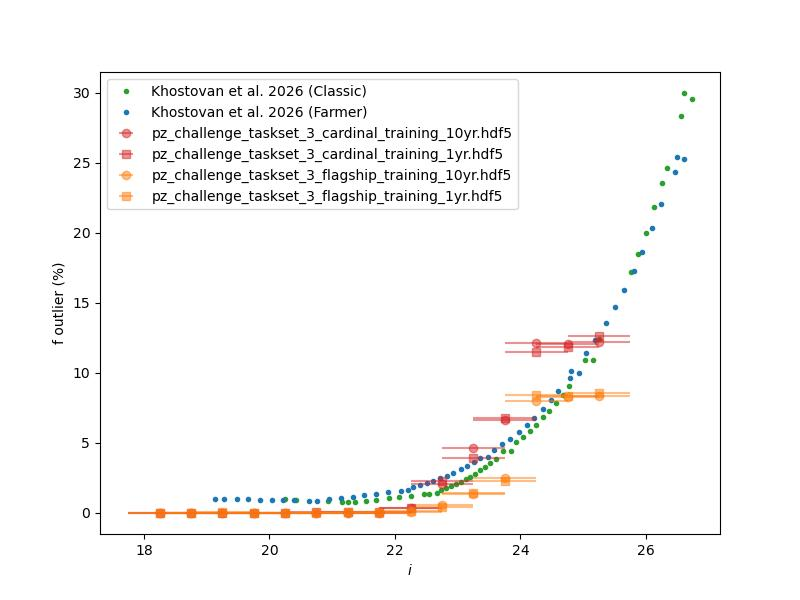
\includegraphics[width=0.45\textwidth]{figures/foutlier_vs_mag_i}    
    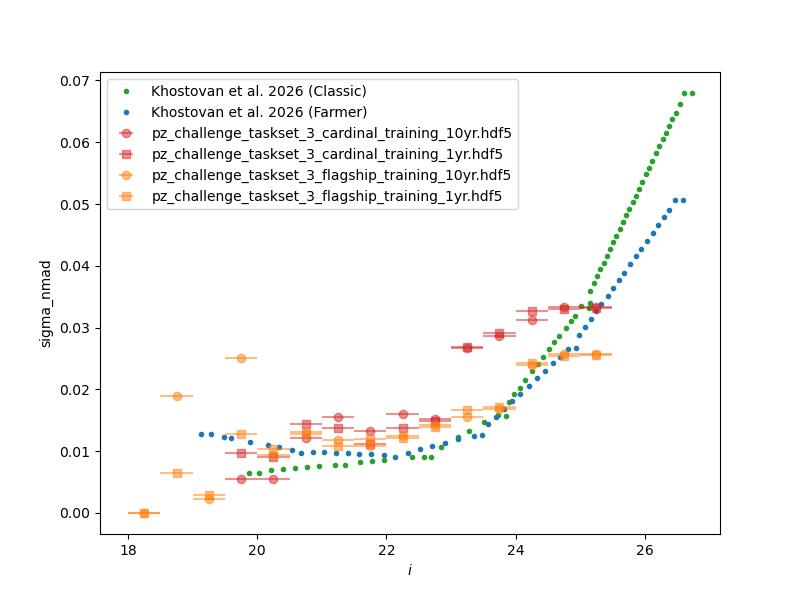
\includegraphics[width=0.45\textwidth]{figures/sigma_nmad_vs_mag_i}
  }
  \caption{\label{fig:manyband_photoz}\small{Performance of the
      multi-band photometric redshift estimates as a function of i-band
      magnitude, showing the outlier fraction (left) and width of the
      median absolute deviation (right).}}
\end{figure*}


\subsection{Emulating unrecognized blending}

In the files for task sets 1--3 we emulate the effect of unrecognized
blending, i.e., two or more objects being detected as a single
object.  Our blending algorithm is relatively simple: we apply a
``friends-of-friends'' matching algorithm with a 1.0 arcsecond linking
length and replace all groups with a single object with the summed fluxes
in each of the bands. 


\begin{figure*}[ht]
  \centerline{
    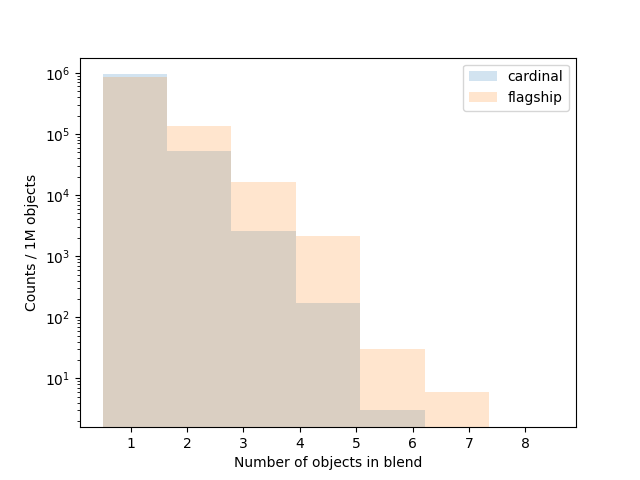
\includegraphics[width=0.45\textwidth]{figures/n_objects_in_blend}    
    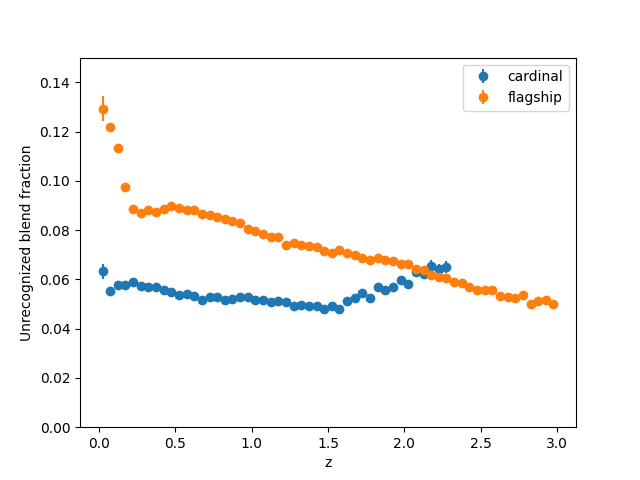
\includegraphics[width=0.45\textwidth]{figures/blend_fractions}
  }
  \centerline{
    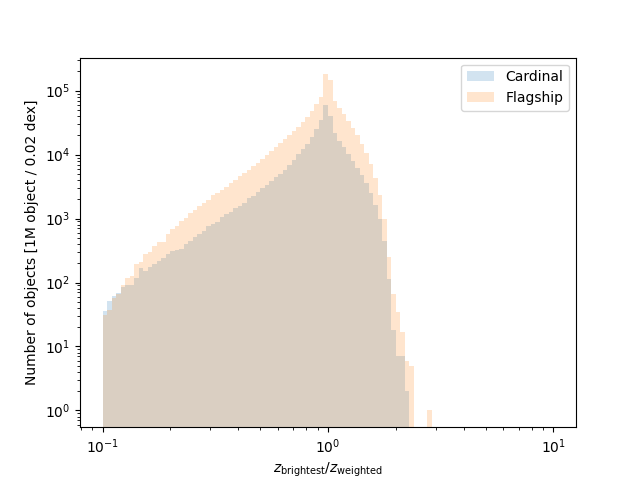
\includegraphics[width=0.45\textwidth]{figures/redshift_ratio}
    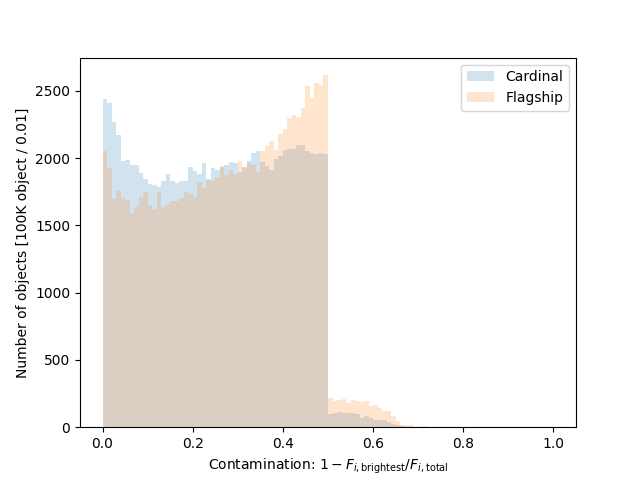
\includegraphics[width=0.45\textwidth]{figures/flux_contamination}
  }
  \caption{\label{fig:blending}\small{Blending behavior.  Top left:
      distribution of the number of objects in each blend.  Top right:
      fraction of objects that are blended as a function of redshift.
      Bottom left: ratio of the redshift of the brightest object in
      the blend to the flux-weighted mean of all the objects.  Bottom
      right: fraction of the total flux in the blend not from the brightest object.}}      
\end{figure*}


\subsection{Field selection and downsampling}
\label{sec:selection_and_downsampling}

The final steps of the data preparation process were to select objects from specific fields
to emulate the ``calibration'' or ``deep-drilling'' fields (DDFs) and to select a sample
from the entire footprint (WFD) to serve as a test dataset.

For the DDFs, we selected sets of objects that passed combined spectroscopic selections.
For the WFD field, we simply downselected 1 million objects from the full dataset.


\section{Data Preparation Tools}
\label{sec:data_preparation_tools}

All of the data preparation was performed using the
\texttt{rail\_projects} and \texttt{rail\_package\_config} packages
for bookkeeping and reproducibility.  The scripts listed in Tab.~\ref{tab:prep_scripts}
comprise the entire production pipeline from the simulation truth catalogs
to the files released with the challenge. 

\begin{table}[ht]
\centering
\caption{\label{tab:prep_scripts}\small Scripts used
  in data preparation.}
\begin{tabular}{lll}
\hline \hline
Script & Command Run & Purpose \\ \hline
  do\_00\_reduce & rail-project reduce & Reduce input truth catalogs \\
  &  & (mag. cut and drop columns) \\ 
do\_01\_build & rail-project build & Build configurations to run \\
  &  & truth-to-observed pipeline \\
do\_02\_t2o & rail-project run truth-to-observed & Run truth-to-observed \\
       &  & pipelines to make degraded catalogs \\
nz\_00\_merge & rail-project merge & Combine spectroscopic selections \\
  nz\_01\_subselect & rail-project subsample & Make ddf/wfd files from catalogs\\
  nz\_02\_export & & clean up files and create output tar file\\
\hline\hline
\end{tabular}
\end{table}


\newpage

\bibliography{nz_challenge.bib}

\end{document}


%  LocalWords:  maketitle fig:pz_redshift_basics includegraphics hdf5
%  LocalWords:  textwidth texttt taskset eac hline hline _lsst pz qp
%  LocalWords:  color_color_redshift_taskset_1_cardinal_10yr github
%  LocalWords:  color_color_redshift_taskset_1_flagship_10yr _1yr.pkl
%  LocalWords:  therailteam2025 iqr schmidt_evaluation_2020 textbf nb
%  LocalWords:  Kullback-Leibler gigaparsecs _subselect newpage zmode
%  LocalWords:  coadded slitless allowbreak _lsst table-io tables_io
%  LocalWords:  texorpdfstring _submission.py _subselect
%  LocalWords:  desicollaboration2025datarelease1dark
